\documentclass[11pt,a4paper]{article}
\usepackage[T1]{fontenc}
\usepackage{lmodern}
\usepackage[margin=26mm]{geometry}
\usepackage{amsmath,amssymb,amsthm,booktabs}
\usepackage[hidelinks]{hyperref}
\usepackage{xcolor,graphicx}
\definecolor{ink}{HTML}{183F47}
\usepackage{titlesec}
\titleformat{\section}{\large\bfseries\color{ink}}{\thesection}{.65em}{}
\titleformat{\subsection}{\normalsize\bfseries\color{ink}}{\thesubsection}{.65em}{}
\newtheorem{thm}{Theorem}[section]
\newtheorem{lem}[thm]{Lemma}
\newtheorem{prop}[thm]{Proposition}
\newtheorem{cor}[thm]{Corollary}
\theoremstyle{remark}
\newtheorem{rem}[thm]{Remark}
\newcommand{\E}{\mathbb E}
\newcommand{\Prob}{\mathbb P}
\newcommand{\Bin}{\operatorname{Bin}}
\newcommand{\Pois}{\operatorname{Pois}}
\setlength{\emergencystretch}{2em}
\title{\color{ink}\bfseries Sharp finite-market prophet inequalities\\for a single threshold}
\author{Anonymous}
\date{November 2026\\[2pt]\small DOI \href{https://doi.org/10.5281/zenodo.24506643}{10.5281/zenodo.24506643}}
\begin{document}
\maketitle
\begin{abstract}
A decision maker sees independent, not necessarily identically distributed values in uniformly random order and accepts the first $k$ that clear one fixed threshold. How large a fraction of the average of the best $\ell$ values in hindsight can such a rule guarantee? We give the exact worst-case fraction at every finite market size $n>\max(k,\ell)$ in three information regimes: the threshold may use all the marginal distributions; it must hit a prescribed probability of filling all $k$ places (the stockout probability); or it must hit a prescribed expected fraction of places filled (the utilisation). Two binomial expectations determine every answer. The utilisation rule at its best target loses nothing against full knowledge of the distributions. The stockout rule loses a positive amount for $k\ge2$, but only of order $n^{-2}$, and we give its leading coefficient. Over all market sizes the stockout target proposed by Arnosti and Ma attains their optimal constant $1-e^{-k}k^k/k!$, which proves their conjecture. Allowing unequal capacities $k\neq\ell$ gives, over all market sizes, the same constant for heterogeneous values as Molina, Gast, Loiseau and Perchet found for identically distributed values. This answers their question for static thresholds. At each finite $n$ heterogeneity strictly lowers the guarantee, by an amount of order $1/n$ with an explicit coefficient. For the distribution-aware value, the matching upper bound comes from a single instance on which every threshold fails. The main theorem extends to weighted rank benchmarks and, for the distribution-aware and stockout rules, to mixtures of random and adversarial arrival order.
\end{abstract}

\section{Introduction}
This section states the problem, explains why it matters, summarises what was known and what is new, and ends with a plan of the paper.

\paragraph{The problem.}
A seller has $k$ identical items and faces $n$ buyers, one at a time, in a random order. Each buyer's value is drawn independently from a known distribution, and different buyers may have different distributions. The seller posts one price before the first buyer arrives, never changes it, and sells to the first $k$ buyers whose value clears it. The same rule describes a firm that fills $k$ posts from $n$ applicants with one fixed hiring bar, or a platform that admits the first $k$ requests above a fixed quality cut-off. We measure the rule against a prophet who sees all values in advance and keeps the best $\ell$ of them, and compare averages per place: the rule's expected total divided by $k$, against the prophet's expected total divided by $\ell$. The question is the worst case of this ratio over all value distributions, at the best choice of the fixed threshold.

\paragraph{Why single thresholds matter.}
A single posted price is the simplest selling mechanism. It treats every buyer alike, it gives no reason to wait or to misreport, and it is easy to explain. It can also be tuned from data. A seller need not know every buyer's distribution, since it is enough to adjust the price until one market-wide statistic, such as how often all the stock sells, reaches a target. The cost of this simplicity is the gap between the best static threshold and the prophet. A finite market, with tens rather than thousands of buyers, is the regime in which managers actually set such targets.

\paragraph{What was known.}
For equal capacities ($k=\ell$) and arbitrarily large markets, Arnosti and Ma \cite{am} showed that a well-chosen static threshold guarantees the fraction
\[
 \gamma_k=1-e^{-k}k^k/k!
\]
of the prophet's value, and that no static threshold guarantees more. Their rule targets a market-wide statistic, the expected utilisation, at the level $\gamma_k$. They showed that no target for the expected number of qualifiers attains $\gamma_k$ for every instance when $k\le4$ \cite[Proposition~1]{am}. In \cite[\S5.2]{am} they conjectured that targeting the probability of selling out at $\Prob(\Pois(k)\ge k)$ also guarantees $\gamma_k$. For $k=1$ this is the rule of Ehsani, Hajiaghayi, Kesselheim and Singla \cite{ehks}. For identically distributed values and finite $n$, Arnosti \cite{blog} and Jiang, Ma and Zhang \cite[Theorem~8 and Corollary~2]{jmz} gave the exact equal-capacity static value. When the arrival order is adversarial, Chawla, Devanur and Lykouris \cite{cdl} found the static-pricing constant, and Jiang, Ma and Zhang \cite[Theorem~6 and equation~(21)]{jmz} gave the exact finite-$n$ value. For unequal capacities and identically distributed values, Molina, Gast, Loiseau and Perchet \cite[Theorem~1.4]{mg} found the limiting static constant with an $O(1/n)$ error. At the end of their \S6 they asked whether such guarantees extend to heterogeneous values in random order.

\paragraph{What is new.}
For every finite $n>\max(k,\ell)$ and heterogeneous independent values in random order:
\begin{itemize}
\item We find the exact worst-case ratio of the best distribution-aware threshold. We also find, as a function of the target, the exact ratio of a threshold calibrated to a stockout probability, and of one calibrated to an expected utilisation (Theorem~\ref{thm:finite}, Proposition~\ref{prop:util}). Identical laws are treated in the same way (Theorem~\ref{thm:finite}(3), Proposition~\ref{prop:iidq}), and the boundary cases $k=n$ or $\ell=n$ are settled (Proposition~\ref{prop:boundary}).
\item These finite values rank the three ways of setting the threshold. The utilisation rule at its best target equals the distribution-aware optimum. The stockout rule is strictly worse for $k\ge2$, by an amount of exact order $n^{-2}$ (Corollary~\ref{cor:gap}). Identical laws are strictly easier, by an amount of exact order $1/n$ (Corollary~\ref{cor:het}).
\item Letting $n$ vary proves the Arnosti--Ma stockout conjecture for every $k$ and every market size (Corollary~\ref{cor:limit}). It also shows that the unequal-capacity constant of Molina et al.\ holds for heterogeneous values in random order, which answers their question for static thresholds.
\end{itemize}
The new ingredient is a comparison of counts at a \emph{common tail probability} rather than at a common mean or utilisation (Lemma~\ref{lem:cross}). It is applied to each applicant's count of qualifying \emph{rivals}, not to the total count of qualifiers. Arnosti and Ma fix the value of a statistic and optimise over the Bernoulli parameters. They show that some optimum uses at most three distinct parameter values \cite[Theorem~4]{am}, and then compare at matched utilisation. A stockout target constrains a tail probability instead. The crossing lemma shows that, at a matched tail, the binomial or Poisson law is worst for both quantities that matter. Combined with their own two-coefficient bound \cite[Lemma~1]{am}, this alone settles the conjecture at every market size. The rival counts are what make the finite values exact. The same lemma also recovers the utilisation case in one line. For the distribution-aware value, the matching upper bound uses one instance, a group of ordinary applicants plus one rare applicant of very high value. The rare value is chosen by a supporting-line argument so that \emph{every} threshold, and every randomisation over thresholds, falls short on that instance.

\paragraph{Plan of the paper.}
Section~\ref{sec:model} fixes the model and notation. Section~\ref{sec:finite} proves the finite-market values: the comparison lemma, the lower bounds, the single hard instance, the boundary cases and the identical-law results. Section~\ref{sec:all} lets the market grow, proves the stockout conjecture and gives the finite costs of the cruder rules. Section~\ref{sec:weights} gives the two extensions. Section~\ref{sec:numerics} reports numerical checks and practical implications, and Section~\ref{sec:discussion} lists limits and open questions.

\subsection{Model and notation}\label{sec:model}
This subsection defines the selection rule, the benchmark and the quantities used throughout.

Let $1\le k,\ell\le n$. The $n$ values $V_1,\dots,V_n$ are independent, nonnegative and integrable, with marginal laws $G=(G_1,\dots,G_n)$. An independent uniform permutation determines their arrival order. A \emph{static threshold} is a pair $(t,h)$ with $t\ge0$ and $h\in[0,1]$. A value above $t$ \emph{qualifies}, and a value equal to $t$ qualifies with probability $h$, by independent coins. The rule accepts the first $k$ qualifiers, or all of them if fewer qualify. The threshold is anonymous: it is the same for every applicant and excludes personalised prices. Write
\[
 W=\frac1k\,\E[\text{sum of accepted values}],\qquad H=\frac1\ell\,\E[\text{sum of the $\ell$ largest values}],
\]
with unfilled places worth zero, and assume $H>0$. Let $p_i=\Prob(i\text{ qualifies})$, let $D$ be the number of qualifiers and let $D_{-i}$ be the number of qualifiers other than $i$. The \emph{stockout probability} is $q=\Prob(D\ge k)$ and the \emph{utilisation} is $\E\min(D,k)/k$.

We study three worst-case values. The \emph{all-static value} is
\[
 C_{n,k,\ell}=\inf_G\ \sup_{t,h}\ W/H .
\]
The \emph{fixed-stockout value} $S_{n,k,\ell}(q)$ is the infimum over $G$ and over all thresholds with stockout probability exactly $q$. The \emph{fixed-utilisation value} $R_{n,k,\ell}(\nu)$ is defined in the same way with utilisation $\nu$. Writing $C^{\rm iid}_{n,k,\ell}$ and $S^{\rm iid}_{n,k,\ell}$ means the infimum is over identical laws $G_1=\dots=G_n$. Every value is an infimum that the hard instances approach but do not attain. Randomising over thresholds does not raise $C_{n,k,\ell}$, because the hard instance of Section~\ref{sec:sharp} defeats every threshold at once.

For $d\ge0$ put
\[
 u(d)=\frac{\min(d,k)}k,\qquad a(d)=\min\!\left(1,\frac{k}{1+d}\right).
\]
Here $u(D)$ is the fraction of places filled, and $a(d)$ is the probability that a qualifying applicant facing $d$ qualifying rivals is accepted, since its rank among the $d+1$ qualifiers is uniform. For $B_m(p)\sim\Bin(m,p)$ define the two binomial expectations
\[
 U_m(p)=\E u(B_m(p)),\qquad A_m(p)=\E a(B_m(p)).
\]
For $m\ge k$ and $0<q<1$, let $p_m(q)$ be the unique solution of $\Prob(B_m(p)\ge k)=q$. For $m\ge k$, $U_m$ is strictly increasing from $0$ to $1$ and $A_m$ is strictly decreasing. We write $b=\ell$. Section~\ref{sec:weights} allows non-integral $b$.

\section{The finite-market values}\label{sec:finite}
This section states the main theorem, proves its lower bounds through a comparison of Bernoulli sums, proves the matching upper bounds through one hard instance, and then treats the utilisation rule, the boundary cases and identical laws.

\begin{thm}[Sharp finite guarantees]\label{thm:finite}
Suppose $n>\max(k,\ell)$, and set $m=n-1$.
\begin{enumerate}
\item For $0<q<1$ the fixed-stockout value is
\begin{equation}\label{eq:q}
 S_{n,k,b}(q)=\min\big\{U_n(p_n(q)),\ (b/k)A_m(p_m(q))\big\}.
\end{equation}
The first branch increases and the second decreases in $q$. The best stockout target is their unique intersection.
\item The all-static value is $C_{n,k,b}=U_m(p_*)$, where $p_*\in(0,1)$ uniquely solves
\begin{equation}\label{eq:balance}
 U_m(p_*)=(b/k)A_m(p_*).
\end{equation}
A threshold attains the guarantee on every instance if it sets $\max_i\Prob(D_{-i}\ge k)=\Prob(B_m(p_*)\ge k)$.
\item For identically distributed values the all-static value is
\begin{equation}\label{eq:iid}
 C^{\rm iid}_{n,k,b}=U_n(b/n).
\end{equation}
It is attained by making each applicant qualify with probability $b/n$.
\end{enumerate}
\end{thm}

For example, with three applicants and two places ($n=3$, $k=\ell=2$) one has $U_2(p)=p$ and $A_2(p)=1-p^2/3$. The all-static value is the root of $p=1-p^2/3$, namely $(\sqrt{21}-3)/2\simeq0.79129$. The best stockout target guarantees $0.78666$. Under identical laws the value rises to $23/27\simeq0.85185$. More generally, when $n=k+1$ one has $U_{n-1}(p)=p$ and $A_{n-1}(p)=1-p^k/(k+1)$, so $C=(b/k)(1-C^k/(k+1))$. This gives $2/3$ at $n=2,k=\ell=1$ and the root of $C^3+4C-4=0$ at $n=4,k=\ell=3$.

\subsection{A tail comparison for Bernoulli sums}
This subsection proves the one probabilistic tool: two counts with the same stockout probability have distribution functions that cross exactly once, at the stockout level.

For a random variable $X$ write $F_X(j)=\Prob(X\le j)$.
\begin{lem}[A common stockout probability]\label{lem:cross}
Let $X$ be a sum of $s\ge k$ independent Bernoulli variables. Let $Y$ be either $B_s(p)$ or a Poisson variable, calibrated so that $\Prob(X\ge k)=\Prob(Y\ge k)\in(0,1)$. Then
\[
 F_X(j)\le F_Y(j)\quad (j<k-1),\qquad
 F_X(k-1)=F_Y(k-1),\qquad F_X(j)\ge F_Y(j)\quad(j>k-1).
\]
Consequently $\E u(X)\ge\E u(Y)$ and $\E a(X)\ge\E a(Y)$.
\end{lem}
\begin{proof}
The probability generating polynomial of $X$ is $\prod_i(1-p_i+p_i z)$. Its roots are real and nonpositive when $0<p_i<1$. Newton's inequalities therefore make the sequence $\Prob(X=j)/\binom{s}{j}$ log-concave. Continuity extends this to $p_i\in\{0,1\}$, and the support of $X$ is an interval of integers. Dividing by a binomial mass multiplies this sequence by a geometric progression. For a Poisson mass the extra factor is, up to a geometric progression, $s!/(s-j)!$, which is itself log-concave. Thus the likelihood ratio $r_j=\Prob(X=j)/\Prob(Y=j)$ is log-concave on the support of $X$ and zero outside it. In particular $\{j:r_j\ge1\}$ is an interval. This is the relative log-concavity familiar from \cite{yu}.

Write $d_j=\Prob(X=j)-\Prob(Y=j)$. By calibration, the sum of $d_j$ over $j<k$ and the sum over $j\ge k$ both vanish. Since both sides of the calibration are positive, some index $j\ge k$ has $\Prob(X=j)\ge\Prob(Y=j)>0$, so $r_j\ge1$ there. Likewise some index below $k$ has $r\ge1$. Suppose the partial sum $\sum_{i\le j}d_i$ were positive for some $j<k-1$. Then some $i\le j$ would have $r_i>1$, and some $i'\in(j,k-1]$ would have $r_{i'}<1$. Together with an index at or above $k$ with $r\ge1$, this contradicts the interval property. Suppose instead the partial sum were negative for some $j\ge k$. Then some entry in $[k,j]$ would have $r<1$, and a later entry would have $r>1$. An earlier index below $k$ has $r\ge1$, which gives the same contradiction. This proves the crossing pattern.

Finally, $\E u(X)=k^{-1}\sum_{j=0}^{k-1}(1-F_X(j))$, which gives the first inequality. Summation by parts gives $\E a(X)=\sum_{j\ge0}\big(a(j)-a(j+1)\big)F_X(j)$. The increments are nonnegative and vanish for $j<k-1$, which gives the second.
\end{proof}

\subsection{Lower bounds and implementation}
This subsection reduces the ratio $W/H$ to two coefficients and bounds each of them by Lemma~\ref{lem:cross}.

Put $e_i=\E(V_i-t)_+$, where $x_+=\max(x,0)$. Given that $i$ qualifies and that $d$ rivals qualify, $i$ is accepted with probability $a(d)$. A positive excess $V_i-t$ forces $i$ to qualify, and $V_i$ is independent of $D_{-i}$. Every accepted value pays the baseline $t$ and possibly an excess. Hence
\begin{equation}\label{eq:decomp}
 W=t\,\E u(D)+\frac1k\sum_i e_i\,\E a(D_{-i}),\qquad H\le t+\frac1b\sum_i e_i .
\end{equation}
The bound on $H$ holds because the $\ell$ largest values sum to at most $\ell t+\sum_i(V_i-t)_+$. Since $t$ and every $e_i$ are nonnegative,
\begin{equation}\label{eq:twocoef}
 \frac WH\ \ge\ \min\Big\{\E u(D),\ \frac bk\min_i\E a(D_{-i})\Big\}.
\end{equation}
The same bound holds against the larger deterministic expression on the right of \eqref{eq:decomp}, and hence against the usual ex-ante relaxation of the prophet.

\emph{Part 1.} At a stockout target $q$, Lemma~\ref{lem:cross} applied to $D$ ($n$ trials) gives $\E u(D)\ge U_n(p_n(q))$. Each $q_i=\Prob(D_{-i}\ge k)$ is at most $q$. If $q_i>0$, the lemma applied to $D_{-i}$ ($m\ge k$ trials) gives $\E a(D_{-i})\ge A_m(p_m(q_i))\ge A_m(p_m(q))$, since $p_m$ increases and $A_m$ decreases. If $q_i=0$, the acceptance is one. This proves the lower bound in part 1.

\emph{Part 2.} Remove an applicant with the smallest qualification probability, and let $D'$ be the count of the others. Swapping one Bernoulli variable for one with a larger parameter shows that $D'$ stochastically dominates every $D_{-i}$. Calibrate the threshold so that $\Prob(D'\ge k)=\Prob(B_m(p_*)\ge k)$. Since $D\ge D'$ and $a$ decreases, the lemma gives
\[
 \E u(D)\ge \E u(D')\ge U_m(p_*),\qquad \min_i\E a(D_{-i})=\E a(D')\ge A_m(p_*).
\]
By \eqref{eq:balance} both coefficients are at least $C_{n,k,b}$. The balance \eqref{eq:balance} is the random-order, finite-market counterpart of the static price of Chawla, Devanur and Lykouris \cite{cdl}, which equates the expected fraction of items sold with the probability that the supply does not sell out.

\emph{Existence of the calibrations.} Lower $t$ from infinity to zero, and at each atom of the laws let the common coin $h$ run from $0$ to $1$. To make this a continuous path, parametrise it by the average qualification probability $\bar p=n^{-1}\sum_ip_i$. This is a quantile of the equally weighted mixture of the marginal laws, split at its atoms. A change of $\bar p$ by $\eta$ changes each $p_i$ monotonically and by at most $n\eta$. The statistics $\Prob(D\ge k)$, $\E u(D)$ and $\max_i\Prob(D_{-i}\ge k)$ are continuous functions of $(p_1,\dots,p_n)$. Each runs from $0$ to $1$ along the path, so every interior target is attained.

\emph{Uniqueness.} $U_m$ increases strictly from $0$ to $1$, and $(b/k)A_m$ decreases strictly from $b/k>0$ to $(b/k)\cdot k/n=b/n<1$. So \eqref{eq:balance} has a unique root in $(0,1)$. The same monotonicity, composed with the increasing maps $q\mapsto p_n(q)$ and $q\mapsto p_m(q)$, gives the unique intersection in part 1.

\emph{Part 3.} For identical laws every applicant qualifies with a common probability $p$, so $D\sim B_n(p)$ and $D_{-i}\sim B_m(p)$. Counting accepted applicants by name gives the exchange identity
\begin{equation}\label{eq:exchange}
 kU_n(p)=npA_m(p).
\end{equation}
At $p=b/n$ the two coefficients in \eqref{eq:twocoef} are both equal to $U_n(b/n)$, which proves the lower bound in part 3.

\subsection{Sharpness: one instance defeats every threshold}\label{sec:sharp}
This subsection builds the instances that show the lower bounds cannot be improved. The main step is a single instance on which no threshold, deterministic or randomised, beats the claimed value.

\emph{Part 1, first branch.} Give every applicant the value one. A calibrated threshold must have $t=1$, and the coin then qualifies each applicant independently with probability $p_n(q)$. The ratio is exactly $U_n(p_n(q))$.

\emph{Part 1, second branch.} Give $m$ applicants the value one. The remaining applicant is worth $M$ with probability $\epsilon<q$ and zero otherwise. A threshold in $(0,1)$, or at zero, qualifies all $m\ge k$ ordinary applicants, so its stockout probability is one. A threshold above one has stockout probability at most $\epsilon<q$. So any calibrated threshold has $t=1$ and a coin $p_\epsilon$ satisfying
\[
 q=\Prob(B_m(p_\epsilon)\ge k)+\epsilon\Prob(B_m(p_\epsilon)=k-1),
\]
and $p_\epsilon\to p_m(q)$ as $\epsilon\to0$. The rare applicant qualifies whenever it is worth $M$, and is then accepted with probability $A_m(p_\epsilon)$. Since $\ell\le m$, $H=1+\epsilon(M-1)/b$. Let $\epsilon M\to\infty$ as $\epsilon\to0$. The rare applicant then dominates both $W$ and $H$, and the ratio tends to $(b/k)A_m(p_m(q))$.

\emph{Part 2.} Put $v=(b/k)A_m$. We first show that there is a $\theta>0$ with
\begin{equation}\label{eq:tangent}
 U_m(p)+\theta v(p)\le (1+\theta)C_{n,k,b}\qquad(0\le p\le1).
\end{equation}
Let $J\sim\Bin(m-1,p)$. Differentiating Bernstein polynomials gives
\[
 U_m'(p)=\frac{m}{k}\Prob(J\le k-1),\qquad
 -A_m'(p)=m\,\E\!\left[\frac{k\,\mathbf1_{J\ge k-1}}{(J+1)(J+2)}\right].
\]
The ratio $U_m'/(-v')$ is non-increasing on $(0,1)$. Indeed, compare its values at $p_1<p_2$ by cross-multiplying. Every index in the numerator is at most $k-1$, and every index in the denominator is at least $k-1$. The binomial likelihood ratio of $p_2$ to $p_1$ increases with the index, so each cross term has the right sign. Choose $\theta=U_m'(p_*)/(-v'(p_*))$. The derivative of $U_m+\theta v$ is then nonnegative to the left of $p_*$ and nonpositive to the right, so its maximum is $U_m(p_*)+\theta v(p_*)=(1+\theta)C_{n,k,b}$.

Now take $m$ applicants with value identically one. Let the exceptional applicant have value $M=1+b\theta/\epsilon$ with probability $\epsilon$ and $1-\delta$ otherwise, for a fixed $0<\delta<1$. Since $\ell\le m$, the benchmark is $H=1+\epsilon(M-1)/b=1+\theta$. Every threshold falls into one of three cases. A threshold above one admits no ordinary applicant ($p=0$). A threshold equal to one admits each ordinary applicant with the coin probability $p$. A threshold below one admits every ordinary applicant ($p=1$). If $p<1$, then $t\ge1$ and the low value $1-\delta$ never qualifies. Ordinary acceptances then contribute at most $U_m(p)$ to $W$. The exceptional applicant contributes its baseline unit only on its rare event, which adds at most $\epsilon/k$. If $p=1$, the accepted values other than $M$ contribute at most $1=U_m(1)$. In every case the excess $M-1$ is earned with probability at most $\epsilon A_m(p)$, even if the threshold thins the high value. So
\[
 W\le U_m(p)+\theta\,v(p)+\epsilon/k\le(1+\theta)C_{n,k,b}+\epsilon/k
\]
by \eqref{eq:tangent}. Hence $W/H\le C_{n,k,b}+\epsilon/(k(1+\theta))$ uniformly over thresholds, and so also over randomisations of thresholds. Letting $\epsilon\to0$ proves the upper bound in part 2.

\emph{Part 3.} Use independent copies of a two-point law: the value $M=1+b\theta/(n\epsilon)$ with probability $\epsilon$, and one otherwise. Here $\theta$ is chosen below. Let $p$ be the qualification probability of a value equal to one. Replacing every rare draw by an ordinary one changes the capped baseline by at most the number of rare draws, which has mean $n\epsilon$. When rare values qualify surely, every other applicant qualifies with probability at least $p$. The rare excess is then at most $(b\theta/k)A_m(p)$. If rare values are thinned, then $p=0$ and the same bound holds. Two or more rare draws have probability $O(\epsilon^2)$, so the benchmark tends to $1+\theta$. The limiting upper curve is therefore $U_n(p)+\theta(b/k)A_m(p)$, and it must be supported at $p=b/n$. Now $U_n'$ averages $\mathbf1_{j\le k-1}$ over $\Bin(n-1,p)$. In contrast, $-A_m'$ averages a nonnegative function $g$, supported on $j\ge k-1$, over $\Bin(n-2,p)$. Raise the latter to degree $n-1$ by Bernstein degree elevation. The coefficient at $j$ becomes $(1-j/(n-1))g(j)+(j/(n-1))g(j-1)$. Its support still starts at $k-1$, because $k<n$. The cross-multiplication argument above therefore shows that the derivative ratio is again non-increasing. Choosing $\theta$ as the ratio at $p=b/n$ and using \eqref{eq:exchange} completes the proof of Theorem~\ref{thm:finite}.\hfill$\square$

\begin{rem}[Continuous laws]\label{rem:continuous}
The interior values of Theorem~\ref{thm:finite} are unchanged if all marginal laws must be continuous. In the part 2 instance, replace each ordinary value by an independent uniform draw on $[1,1+\delta]$. Replace the low and high exceptional values by uniform draws on $[1-2\delta,1-\delta]$ and $[M,M+\delta]$. Every threshold still gives the ordinary applicants a common probability $p$, and if $p<1$ the low band cannot qualify. The baseline changes by $O(\delta+\epsilon)$ uniformly in the threshold, and the high event still has conditional acceptance at most $A_m(p)$. Treat the two bands of the part 3 instance in the same way. For part 1, the all-ordinary instance has common probability $p_n(q)$ and scores within $O(\delta)$ of its limit. In the exceptional part 1 instance, spread the ordinary values on $[1,1+\delta]$ and the high value on $[M,M+\delta]$ as in part 2, and replace the value zero by a uniform draw on $[0,\delta]$. For small $\epsilon$ a calibrated threshold lies in the ordinary band, where the stockout equation keeps the displayed form. Letting $\delta\to0$ proves the claim.
\end{rem}

\subsection{Calibrating utilisation instead of stockout}
This subsection shows that the utilisation statistic, the one Arnosti and Ma used, loses nothing at finite $n$ when its target is set correctly.

\begin{prop}[Utilisation targets]\label{prop:util}
Suppose $n>\max(k,\ell)$, set $m=n-1$, and let $0<\nu<1$. The fixed-utilisation value is
\[
 R_{n,k,b}(\nu)=\min\big\{\nu,\ (b/k)A_m(U_m^{-1}(\nu))\big\}.
\]
Its maximum over $\nu$ equals the all-static value $C_{n,k,b}$, attained at $\nu=C_{n,k,b}$.
\end{prop}
\begin{proof}
\emph{Lower bound.} The utilisation coefficient in \eqref{eq:twocoef} equals $\nu$. Fix $i$. Since $D_{-i}\le D$, $\E u(D_{-i})\le\nu<1$, so $\Prob(D_{-i}\ge k)<1$. If this probability is zero, the acceptance is one. Otherwise let $Y=B_m(p_m(\Prob(D_{-i}\ge k)))$. Lemma~\ref{lem:cross} gives $\E u(D_{-i})\ge\E u(Y)$ and $\E a(D_{-i})\ge\E a(Y)$. The first inequality says that $Y$'s binomial parameter is at most $U_m^{-1}(\E u(D_{-i}))\le U_m^{-1}(\nu)$. Since $A_m$ decreases, $\E a(D_{-i})\ge A_m(U_m^{-1}(\nu))$.

\emph{Upper bound.} If every value is one, a calibrated threshold sits at one with a coin $h$ satisfying $U_n(h)=\nu$, and the ratio is $\nu$. In the second instance of part 1, $m$ values are one and the rare value is $M$ with probability $\epsilon$. Thresholds below one give utilisation one, and thresholds above one give utilisation at most $\epsilon/k$. So for small $\epsilon$ a calibrated threshold sits at one with a coin $p_\epsilon\to U_m^{-1}(\nu)$. Then, as before, the ratio tends to $(b/k)A_m(U_m^{-1}(\nu))$.

\emph{Optimum.} The first branch increases in $\nu$ and the second decreases. At $\nu=C_{n,k,b}=U_m(p_*)$ the second branch is $(b/k)A_m(p_*)=C_{n,k,b}$ by \eqref{eq:balance}.
\end{proof}
Arnosti and Ma \cite[Lemma~2]{am} proved the binomial extremality at matched utilisation for the full count $D$ by a two-coordinate exchange argument. Lemma~\ref{lem:cross} gives it in one line. Applying it to the rival counts $D_{-i}$, rather than to $D$, is what makes the finite value exact. Their rule targets the limit $\gamma_k$. At finite $n$ the best target is $C_{n,k,k}\ge\gamma_k$.

\subsection{The boundary cases}
This subsection completes Theorem~\ref{thm:finite} when one capacity equals the market size.

\begin{prop}[Full-market capacities]\label{prop:boundary}
Let $n\ge1$ and $0<q<1$.
\begin{enumerate}
\item $C_{n,n,\ell}=C^{\rm iid}_{n,n,\ell}=\ell/n$ for $1\le\ell\le n$, and $C_{n,k,n}=C^{\rm iid}_{n,k,n}=1$ for $1\le k\le n$.
\item $S_{n,n,b}(q)=\min\{q^{1/n},\,b/n\}$ for $1\le b\le n$.
\item $S_{n,k,n}(q)=U_n(p_n(q))$ for $1\le k<n$.
\end{enumerate}
\end{prop}
\begin{proof}
(1) With $k=n$, accept every value ($t=0$, $h=1$). Then $W=\E\sum_iV_i/n$, while the $\ell$ largest values sum to at most $\sum_iV_i$, so $W/H\ge\ell/n$. For sharpness, let one value be $M$ with probability $\epsilon$ and zero otherwise, with the others identically zero. Any threshold that ever accepts the high value gives $W=\epsilon M/n$ against $H=\epsilon M/\ell$. Under identical laws, use independent copies of this two-point law. Then $W\le\E\sum_iV_i/n=\epsilon M$ and $H\ge n\epsilon(1-\epsilon)^{n-1}M/\ell$, so the ratio is at most $\ell/n+O(\epsilon)$. With $\ell=n$, accept the first $k$ arrivals ($t=0$, $h=1$). In random order each value is accepted with probability $k/n$, so $W=\E\sum_iV_i/n=H$. Values identically one give ratio one, so no instance can force a better constant than one.

(2) With $k=n$, $a(d)=1$ for every $d\le n-1$, so every qualifier is accepted. Stockout means that every applicant qualifies, so $\prod_ip_i=q$. By the arithmetic--geometric mean inequality, $\E u(D)=n^{-1}\sum_ip_i\ge q^{1/n}$. By \eqref{eq:twocoef}, $W/H\ge\min\{q^{1/n},b/n\}$. Values identically one force $p_i=q^{1/n}$ and give the ratio $q^{1/n}$. For the branch $b/n$, take $n-1$ values identically one and one value equal to $M$ with probability $\epsilon<q$ and zero otherwise. A threshold above zero admits the exceptional applicant only on its rare event, so its stockout probability is at most $\epsilon<q$. A calibrated threshold therefore sits at zero, and every value equal to one or to $M$ is accepted. Then $W=(n-1+\epsilon M)/n$, while $H=(\epsilon M+O(1))/b$, since the high value is among the $b$ largest whenever it occurs. So the ratio tends to $b/n$ as $\epsilon M\to\infty$.

(3) With $\ell=n$ and $k<n$, $a(d)\ge k/n$ for $d\le n-1$, so $(n/k)\E a(D_{-i})\ge1\ge\E u(D)$. Lemma~\ref{lem:cross} gives $\E u(D)\ge U_n(p_n(q))$. Values identically one attain this.
\end{proof}
The identical-law formula \eqref{eq:iid} is consistent with part 1, since $U_n(\ell/n)=\ell/n$ when $k=n$ and $U_n(1)=1$. Proposition~\ref{prop:iidq} below covers the identical-law stockout value at the boundary. The extensions of Section~\ref{sec:weights} and Remark~\ref{rem:continuous} are claimed only for the interior range $n>\max(k,\ell)$.

\subsection{Stockout targets under identical laws}
This subsection gives the identical-law analogue of part 1, which completes the comparison of information regimes.

\begin{prop}[Identical laws at a fixed target]\label{prop:iidq}
Let $1\le k,\ell\le n$, $n\ge2$ and $0<q<1$, and write $m=n-1$. Then
\[
 S^{\rm iid}_{n,k,b}(q)=\min\big\{U_n(p_n(q)),\ (b/k)A_m(p_n(q))\big\}.
\]
For $\ell<n$ the maximum over $q$ is $C^{\rm iid}_{n,k,b}=U_n(b/n)$, attained at $q=\Prob(B_n(b/n)\ge k)$. For $\ell=n$ the supremum is $1$, approached as $q\to1$.
\end{prop}
\begin{proof}
Under identical laws a calibrated threshold gives every applicant the qualification probability $p=p_n(q)$, so $D\sim B_n(p)$ and $D_{-i}\sim B_m(p)$. The lower bound follows from \eqref{eq:twocoef}. Values identically one attain the first branch. For the second, use independent copies of the law that equals $M=1+\epsilon^{-2}$ with probability $\epsilon$ and one otherwise. Thresholds below one give stockout one, and thresholds above one give stockout at most $\Prob(B_n(\epsilon)\ge k)<q$ for small $\epsilon$. So a calibrated threshold sits at one, and every applicant qualifies with probability exactly $p$. By \eqref{eq:decomp}, $W=U_n(p)+n\epsilon(M-1)A_m(p)/k$. The benchmark is $H=1+(M-1)\E\min(R,\ell)/\ell$ with $R\sim\Bin(n,\epsilon)$, and $\E\min(R,\ell)=n\epsilon+O(\epsilon^2)$. Hence $W/H\to(b/k)A_m(p)$. The two branches cross where $U_n(p)=(b/k)A_m(p)$, which by \eqref{eq:exchange} means $p=b/n$.
\end{proof}
The optimum $p=b/n$ is the quantile rule of \cite[Proposition~6.1]{mg}, analysed there asymptotically for every $\ell$, and for $\ell=k$ the exact finite optimum of \cite[Theorem~8]{jmz}. New here are the exact finite curve in $q$ and the exact finite value for $\ell\neq k$. Under identical laws, then, the stockout statistic loses nothing at its best target. The losses in Section~\ref{sec:all} come from heterogeneity.

\paragraph{The price of a stockout target.}
For $k=1$, $\E u(D)=\Prob(D\ge1)=q$, so the stockout rule coincides with the utilisation rule and $\max_qS_{n,1,b}(q)=C_{n,1,b}$. For $k\ge2$ the inequality $\max_qS_{n,k,b}(q)<C_{n,k,b}$ is strict. To see this, put $q=\Prob(B_m(p_*)\ge k)$ and compare $B_m(p_*)$, padded by one trial with parameter zero, with $B_n(p_n(q))$. Equal utilisation would force equal distribution functions through $k-1$, by the crossing pattern of Lemma~\ref{lem:cross}. Since $k\ge2$, this includes equal masses at zero and one. For Bernoulli parameters $r_i<1$, the mass at zero is $\prod_i(1-r_i)$. The ratio of the mass at one to the mass at zero is $\sum_ir_i/(1-r_i)=\sum_i\big((1-r_i)^{-1}-1\big)$. Matching both masses with the binomial would make the arithmetic and geometric means of $(1-r_i)^{-1}$ equal. That forces all $r_i$ to be equal, which is false because one of them is zero. So the first branch of \eqref{eq:q} is strictly below $C_{n,k,b}$ at this $q$, while the second branch equals it. By the monotonicity of the branches, the optimal intersection lies at a larger $q$, where the second branch is strictly smaller than $C_{n,k,b}$.

\section{All market sizes and the stockout conjecture}\label{sec:all}
This section lets the market size vary. It proves the Arnosti--Ma conjecture and answers the question of Molina et al., and then measures how fast the finite values approach their limit.

Let $Z_\lambda\sim\Pois(\lambda)$. Write $U(\lambda)=\E u(Z_\lambda)$ and $A(\lambda)=\E a(Z_\lambda)$, and choose $\lambda_q$ by $\Prob(Z_{\lambda_q}\ge k)=q$.
\begin{cor}\label{cor:limit}
Fix $k$, $\ell$ and $0<q<1$. Over all market sizes $n\ge\max(k,\ell)$, the worst-case ratio at stockout target $q$ is
\[
 \min\{U(\lambda_q),\,(b/k)A(\lambda_q)\}.
\]
Its unique maximum over $q$ occurs at $\lambda_q=b$. The all-static value and the identical-law all-static value over all market sizes both equal
\[
 \frac1k\E\min\{\Pois(b),k\}=\frac1k\sum_{j=1}^k\Prob(\Pois(b)\ge j).
\]
\end{cor}
\begin{proof}
Compare the full and rival counts directly with Poisson laws matched at the same stockout probability, using Lemma~\ref{lem:cross}. Counts that cannot reach $k$ have acceptance one. This proves the lower bound $\min\{U(\lambda_q),(b/k)A(\lambda_q)\}$ at every $n$. For the upper bound, $s\,p_s(q)\to\lambda_q$ as $s\to\infty$: for any small $\eta>0$, the binomial tails at $p=(\lambda_q\pm\eta)/s$ bracket $q$ for large $s$, by the law of small numbers. Bounded test functions then carry \eqref{eq:q} to the limit. The Poisson shift identity $\E[Zf(Z)]=\lambda\E f(Z+1)$ gives $kU(\lambda)=\lambda A(\lambda)$. Since $U$ increases and $(b/k)A=bU(\lambda)/\lambda$ strictly decreases, the maximum is at $\lambda=b$. Finally, \eqref{eq:iid} tends to $U(b)$ as $n\to\infty$, which bounds the heterogeneous all-static value from above as well.
\end{proof}
At $b=k$, the shift identity gives $\E(k-Z_k)_+=k\Prob(Z_k=k)$, so $U(k)=1-e^{-k}k^k/k!=\gamma_k$. The optimal target $\Prob(Z_k\ge k)$ is exactly the stockout probability conjectured in \cite[\S5.2]{am}. Hence the Arnosti--Ma rule guarantees $\gamma_k$ on every instance, for every market size and every $k$. The case $k=1$ is the theorem of \cite{ehks}. For the conjecture alone the rival counts are not needed. Arnosti and Ma's bound \cite[Lemma~1]{am} gives the ratio as at least $\min\{\E u(D),\E a(D)\}$. Lemma~\ref{lem:cross} with a Poisson comparison bounds both terms below by $U(k)=A(k)=\gamma_k$ at the conjectured target. For unequal capacities, Corollary~\ref{cor:limit} agrees with the identical-law limit of \cite[Theorem~1.4]{mg}, since $\Prob(\mathrm{Gamma}(j,1)\le\ell)=\Prob(\Pois(\ell)\ge j)$. This answers their question for static thresholds. Every rule in these results keeps the same threshold throughout the arrival sequence.

\subsection{The finite cost of coarser information}\label{sec:secondorder}
This subsection measures, for large $n$, how much the stockout rule loses against the distribution-aware optimum, and how much heterogeneity loses against identical laws. The first loss is of order $n^{-2}$, the second of order $1/n$.

Throughout, $U$ and $A$ are the Poisson functions of Section~\ref{sec:all}, $Z\sim\Pois(b)$, $c=\E u(Z)$ is the limiting value, and $k$ and $b\ge1$ are fixed while $n\to\infty$ with $n>\max(k,b)$.

\begin{cor}\label{cor:gap}
The cost of a stockout target is
\[
 C_{n,k,b}-\max_q S_{n,k,b}(q)
 =\frac{b\,\E(k-1-Z)_+}{2k}\,
   \frac{\Prob(Z>k)}{c}\,\frac{1}{n^2}+O_{k,b}(n^{-3}).
\]
The coefficient of $n^{-2}$ is positive for $k\ge2$. For $k=1$ the two values are equal at every $n$.
\end{cor}

\begin{cor}\label{cor:het}
At every $n$, $C_{n,k,b}<C^{\rm iid}_{n,k,b}$. Moreover,
\[
 C^{\rm iid}_{n,k,b}-C_{n,k,b}=\frac{b\,\Prob(Z<k)\,\Prob(Z>k)}{k\,c}\,\frac1n+O_{k,b}(n^{-2}).
\]
\end{cor}

\begin{proof}[Proof of the strict inequality in Corollary~\ref{cor:het}]
Take $p_0=b/n$. By \eqref{eq:exchange}, $U_n(p_0)=(b/k)A_{n-1}(p_0)$. Adding one trial to $B_{n-1}(p_0)$ strictly increases its expected capped count, so $U_{n-1}(p_0)<U_n(p_0)=(b/k)A_{n-1}(p_0)$. By \eqref{eq:balance}, $p_*>p_0$. Since $A_{n-1}$ strictly decreases, $C_{n,k,b}=(b/k)A_{n-1}(p_*)<(b/k)A_{n-1}(p_0)=C^{\rm iid}_{n,k,b}$.
\end{proof}

\paragraph{Analytic set-up.}
Both expansions rest on one fact: a binomial expectation of a function of a capped count is an analytic function of the inverse number of trials and of the mean. Write $\sigma$ for the inverse number of trials and $y$ for the mean. For fixed $j$, the binomial mass at $j$ has the analytic continuation
\[
 \frac{y^j}{j!}\prod_{i=0}^{j-1}(1-i\sigma)\,(1-\sigma y)^{1/\sigma-j},
\]
using $\log(1-\sigma y)/\sigma=-y+O(\sigma)$ near $\sigma=0$. Let $f$ be the utilisation $u$ or the stockout indicator $\mathbf 1_{d\ge k}$. Each is a constant plus a finite combination of the masses at $j<k$, so its binomial expectation $\widetilde f(\sigma,y)$ is analytic near $(0,b)$. The acceptance function is covered as well, because $A_m(p)=kU_{m+1}(p)/((m+1)p)$ for $p>0$. The probability generating function is $\exp(y(z-1))\big(1-\sigma y^2(z-1)^2/2+O(\sigma^2)\big)$, so
\begin{equation}\label{eq:sigma}
 \widetilde f(\sigma,y)=f^{\rm P}(y)-\tfrac12\sigma y^2\,(f^{\rm P})''(y)+O(\sigma^2),
\end{equation}
where $f^{\rm P}(y)=\E f(Z_y)$ is the Poisson value. For the utilisation, $U'(y)=\Prob(Z_y<k)/k$ and $U''(y)=-\Prob(Z_y=k-1)/k$. Also put $T_0(y)=(b/k)A(y)=bU(y)/y$. The derivative of $U-T_0$ at $b$ is $U(b)/b=c/b>0$. The Poisson shift identity gives $c-bU'(b)=\Prob(Z>k)$.

In both proofs the finite intersection is unique by Theorem~\ref{thm:finite}. The analytic implicit function theorem gives a root near $b$ for all large $n$, so the two coincide.

\begin{proof}[Proof of Corollary~\ref{cor:gap}]
Parametrise the stockout level by $Q(x)=\Prob(Z_x\ge k)$, which has $Q'(x)=\Prob(Z_x=k-1)>0$. Let $s=1/m$. Let $L(s,x)=U_m(p_m(Q(x)))$ and $T(s,x)=(b/k)A_m(p_m(Q(x)))$. By the set-up and the analytic implicit function theorem, the calibrated mean $y(s,x)$ is analytic near $(0,b)$, and so are $L$ and $T$. At $s=0$ they equal $U(x)$ and $T_0(x)$. Implicit differentiation of the stockout equation gives $\partial_sy(0,x)=x^2Q''(x)/(2Q'(x))$, and then \eqref{eq:sigma} gives
\[
 L_s(0,x)=\frac{x^2}{2}\!\left(U'(x)\frac{Q''(x)}{Q'(x)}-U''(x)\right)
         =\frac{x}{2k}\E(k-1-Z_x)_+ ,
\]
using $U''=-Q'/k$ and $Q''/Q'=(k-1)/x-1$.

Set $s=1/(n-1)$ and $s'=1/n$. The all-static value is the ordinate where $L(s,\cdot)$ meets $T(s,\cdot)$. The best stockout value is the ordinate where $L(s',\cdot)$ meets the same $T(s,\cdot)$, because the full count has $n$ trials and the rival count $n-1$. Write $\Gamma(r,s)$ for the ordinate at the root of $L(r,x)=T(s,x)$ near $x=b$. It is analytic, and
\[
 \Gamma_r(0,0)=\frac{-T_0'(b)}{U'(b)-T_0'(b)}\,L_s(0,b)=\frac{\Prob(Z>k)}{c}\,L_s(0,b).
\]
Hence $\Gamma(s,s)-\Gamma(s',s)=(s-s')\,[\Gamma_r(0,0)+O(s)]$, and $s-s'=n^{-2}+O(n^{-3})$. For $k\ge2$, $\E(k-1-Z)_+>0$, so the coefficient is positive. For $k=1$ the two values coincide by the remark at the end of Section~\ref{sec:finite}.
\end{proof}

\begin{proof}[Proof of the expansion in Corollary~\ref{cor:het}]
Let $s=1/n$ and write the qualification probability as $p=y/n$. By \eqref{eq:sigma}, $C^{\rm iid}_{n,k,b}=U_n(b/n)=c-\tfrac12 sb^2U''(b)+O(s^2)$. For the heterogeneous value, $U_{n-1}(y/n)$ has $n-1$ trials and mean $y(1-s)$, and $1/(n-1)=s+O(s^2)$. So
\begin{align*}
 U_{n-1}(y/n)&=U(y)-s\,yU'(y)-\tfrac12sy^2U''(y)+O(s^2),\\
 \frac bkA_{n-1}(y/n)=\frac byU_n(y/n)&=T_0(y)-\tfrac12 s\,b\,yU''(y)+O(s^2).
\end{align*}
Let $\Psi(s,y)$ be the difference of these two expressions, so that \eqref{eq:balance} reads $\Psi(s,y)=0$. Then $\partial_y\Psi(0,b)=c/b$ and $\partial_s\Psi(0,b)=-bU'(b)$. So the root is $y=b+s\,b^2U'(b)/c+O(s^2)$. Evaluating the second expression at the root gives
\[
 C_{n,k,b}=c+s\Big[\big(U'(b)-c/b\big)\frac{b^2U'(b)}{c}-\tfrac12 b^2U''(b)\Big]+O(s^2).
\]
Subtracting this from the expansion of $C^{\rm iid}_{n,k,b}$ gives $s\,bU'(b)\,(c-bU'(b))/c$. This equals $s\,b\Prob(Z<k)\Prob(Z>k)/(kc)$.
\end{proof}


\section{Two extensions}\label{sec:weights}
This section shows that Theorem~\ref{thm:finite} survives two changes to the model: a weighted benchmark and partly adversarial arrival order. Both are claimed for the interior range $n>\max(k,\ell)$.

\paragraph{Weighted order statistics.}
Let the benchmark be $H=\E\sum_{j=1}^n\omega_jV_{(j)}$, where $V_{(1)}\ge\dots\ge V_{(n)}$, $\omega_j\ge0$, $\sum_j\omega_j=1$ and $\omega_1=\max_j\omega_j$. Then Theorem~\ref{thm:finite} holds for $k<n$ with $b=1/\omega_1<n$, and with no other dependence on the weights. Indeed, $H\le t+\omega_1\sum_ie_i$ proves all the lower bounds. The all-ones instance is unchanged. On the part 2 instance the benchmark is $1+\theta-(1-\epsilon)\omega_n\delta$, which tends to $1+\theta$ as $\delta\to0$. In the exceptional part 1 instance, the rare high value carries the coefficient $\omega_1$. In the identical-law two-point instance, counting single rare draws again gives a benchmark tending to $1+\theta$. Uniform weights on all $n$ ranks give the boundary $b=n$, covered by Proposition~\ref{prop:boundary}. Molina et al.\ consider weighted ranks for online selection in \cite[\S7.1]{mg}.

\paragraph{Imperfectly random order.}
Fix $0\le\rho\le1$. Independently of the values, the arrival order is a uniform permutation with probability $1-\rho$ and an arbitrary fixed permutation with probability $\rho$. The guarantee must hold for every choice of the fixed permutation. In parts 1 and 2 of Theorem~\ref{thm:finite}, replace every $A_m(p)$ by
\[
 A_m^{(\rho)}(p)=(1-\rho)A_m(p)+\rho\,\Prob(B_m(p)<k).
\]
The resulting values are exact in this model. On the fixed-order event, a qualifying applicant is certainly served when fewer than $k$ rivals qualify. Lemma~\ref{lem:cross} controls the uniform component, and matching the tail controls the fixed-order component, because $\Prob(D_{-i}<k)=1-q_i$. The lower-bound proof therefore applies with this replacement. In both exceptional upper instances, put the exceptional applicant last in the fixed permutation. Its fixed-order acceptance probability is then exactly $\Prob(B_m(p)<k)$ when it qualifies. The derivative of the new decreasing branch adds a nonnegative multiple of $\mathbf1_{J=k-1}$ before averaging, so the support argument behind \eqref{eq:tangent} still applies. This proves sharpness against the same fixed permutation at every threshold. The case $\rho=1$, $b=k$ recovers the finite adversarial-order value \cite[equation~(21)]{jmz}. The mixture parameter specifies an arrival law and makes no claim about how real applicants order themselves.

\section{Numerical checks and implications}\label{sec:numerics}
This section tabulates the values, states what they mean for a practitioner, and describes the accompanying verification programs.

\begin{figure}[ht]
\centering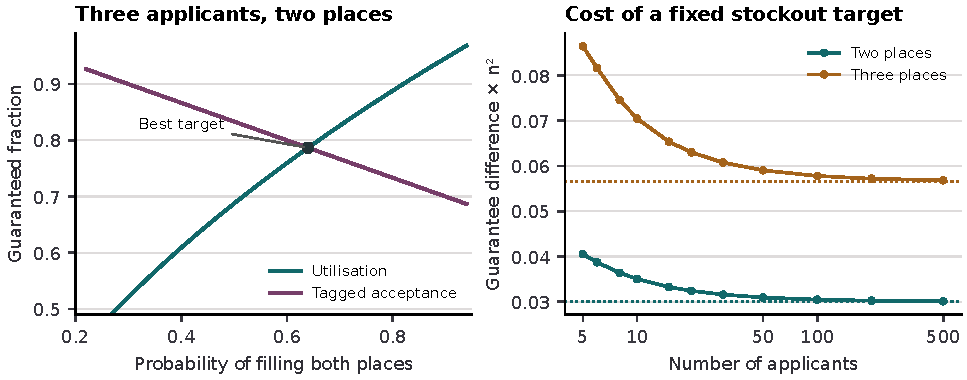
\includegraphics[width=\linewidth]{figures/frontier.pdf}
\caption{Left: three applicants and two places. The guarantee at each stockout target is the lower of the two curves, and the best target is their crossing. Right: the difference between the distribution-aware and best stockout guarantees, multiplied by $n^2$, for equal capacities $k=\ell=2$ and $k=\ell=3$. The dotted lines are the limits from Corollary~\ref{cor:gap}.}
\end{figure}

\begin{table}[ht]
\centering\small
\begin{tabular}{rrr rr c rr}
\toprule
 & & & \multicolumn{2}{c}{Stockout rule} & All static & \multicolumn{2}{c}{Identical laws}\\
$n$&$k$&$\ell$&best $q$&value&(= best utilisation)&value&best $q$\\
\midrule
2&1&1&0.66667&0.66667&0.66667&0.75000&0.75000\\
3&2&2&0.64002&0.78666&0.79129&0.85185&0.74074\\
6&2&4&0.95929&0.97761&0.97782&0.99040&0.98217\\
10&3&3&0.58255&0.79285&0.79356&0.81322&0.61722\\
20&2&2&0.59582&0.73414&0.73422&0.74334&0.60825\\
50&2&2&0.59465&0.73119&0.73120&0.73482&0.59952\\
\bottomrule
\end{tabular}
\caption{Exact finite values. ``All static'' is $C_{n,k,\ell}$, which by Proposition~\ref{prop:util} is also attained by the utilisation target $\nu=C_{n,k,\ell}$. The identical-law value is $C^{\rm iid}_{n,k,\ell}=U_n(\ell/n)$, attained at the stockout target in the last column (Proposition~\ref{prop:iidq}). Over all market sizes with $k=\ell$, the values approach $\gamma_k$ and the best stockout targets approach $\Prob(\Pois(k)\ge k)$: $0.63212$, $0.59399$, $0.57681$ for $k=1,2,3$.}
\end{table}

\paragraph{Implications.}
A seller who knows only the market size and the capacities, and who can see from period to period whether the stock ran out, can tune one price until stockout occurs with the probability $q^*$ in the table. This guarantees within $O(n^{-2})$ of what full knowledge of every buyer's distribution would allow. For $k=\ell=2$ the shortfall is about $0.030/n^2$, which is below $10^{-4}$ once $n\ge20$. A seller who can see the average fraction of stock sold can tune it to $C_{n,k,\ell}$ and lose nothing. Neither statistic can recover the advantage of identically distributed buyers, which is of order $1/n$ and is about $0.18/n$ for $k=\ell=2$. The stockout guarantee has a kink at $q^*$, so a misestimated target costs at first order: below $q^*$ the guarantee falls along the utilisation branch, and above it along the acceptance branch. In the large-market limit with $k=\ell$, the best stockout target is $\Prob(\Pois(k)\ge k)$. This is slightly above one half for large $k$, as Arnosti and Ma observed.

\paragraph{Verification.}
The verification program \texttt{verify.py} checks, in exact rational arithmetic, the crossing pattern of Lemma~\ref{lem:cross} on 585 rational Bernoulli profiles, and \eqref{eq:decomp} and \eqref{eq:twocoef} against direct enumeration of values, tie coins and arrival orders on 12 product laws. In floating point it spot-checks the supporting inequality \eqref{eq:tangent} on a grid for 650 parameter triples. The program \texttt{check\_extensions.py} evaluates the order-mixture hard instances at 189 parameter profiles. It also compares the scaled finite gap of Corollary~\ref{cor:gap} with its coefficient at five parameter pairs. The program \texttt{check\_additions.py} works at 50 significant digits. It checks Propositions~\ref{prop:boundary} and~\ref{prop:iidq}, Corollary~\ref{cor:het} (to five or more significant digits after extrapolation at six parameter pairs) and the values in the table. These calculations check the formulas. The proofs are the inequalities and limiting hard instances above.

\section{Limits and open questions}\label{sec:discussion}
This section records what the results do not cover.

The results concern one anonymous threshold with a common tie coin, independent values and a uniformly random arrival order independent of the values. Personalised prices, adaptive thresholds, dependent values and order chosen in response to the values are all outside the model. ``Sharp'' means that the stated value is the infimum over instances. The hard instances use a rare, very valuable applicant, so a benchmark that limits the dispersion of the best value, as in Loiseau et al.\ \cite{lmpsv}, can give larger values. Three questions remain open. The first is the exact finite value of the expected-demand rule, which Arnosti and Ma showed to be suboptimal for $k\le4$. The second is the finite cost of stockout targets under the order mixtures of Section~\ref{sec:weights}. The third concerns adaptive policies. The gap between the static values here and the optimal adaptive values is known only in limits; for identical laws, see the related analysis of adaptive multi-unit limits in \cite{epiid}.

\paragraph{AI-use statement.}
This manuscript was prepared with substantial assistance from AI systems, which drafted proofs, wrote the verification programs and carried out an internal review. The verification programs are released with the paper. The results have not been refereed.

\begin{thebibliography}{10}\small
\bibitem{epiid} Anonymous. (2026). \emph{Asymptotic i.i.d. prophet inequalities: Fixed-capacity limits and certified two-unit bounds}. Evidence Press. \url{https://doi.org/10.5281/zenodo.23404235}
\bibitem{blog} Arnosti, N. (2020, October 2). \emph{IID prophet inequalities}. \url{https://nickarnosti.com/blog/iidprophet/}
\bibitem{am} Arnosti, N., \& Ma, W. (2023). Tight guarantees for static threshold policies in the prophet secretary problem. \emph{Operations Research, 71}(5), 1777--1788. \url{https://doi.org/10.1287/opre.2022.2419}
\bibitem{cdl} Chawla, S., Devanur, N., \& Lykouris, T. (2024). Static pricing for multi-unit prophet inequalities. \emph{Operations Research, 72}(4), 1388--1399. \url{https://doi.org/10.1287/opre.2023.0031}
\bibitem{ehks} Ehsani, S., Hajiaghayi, M., Kesselheim, T., \& Singla, S. (2018). Prophet secretary for combinatorial auctions and matroids. In \emph{Proceedings of the Twenty-Ninth Annual ACM--SIAM Symposium on Discrete Algorithms} (pp.~700--714). \url{https://doi.org/10.1137/1.9781611975031.46}
\bibitem{jmz} Jiang, J., Ma, W., \& Zhang, J. (2026). Tightness without counterexamples: A new approach and new results for prophet inequalities. \emph{Mathematics of Operations Research, 51}(2), 956--987. \url{https://doi.org/10.1287/moor.2023.0221}
\bibitem{lmpsv} Loiseau, P., Molina, M., Perchet, V., Perez-Salazar, S., \& Verdugo, V. (2026). \emph{Kernel methods for refined prophet inequalities} [Preprint]. arXiv:2608.08662. \url{https://arxiv.org/abs/2608.08662}
\bibitem{mg} Molina, M., Gast, N., Loiseau, P., \& Perchet, V. (2025). Prophet inequalities: Competing with the top $\ell$ items is easy. In \emph{Proceedings of the 2025 Annual ACM--SIAM Symposium on Discrete Algorithms} (pp.~1270--1307). \url{https://doi.org/10.1137/1.9781611978322.38}
\bibitem{yu} Yu, Y. (2010). Relative log-concavity and a pair of triangle inequalities. \emph{Bernoulli, 16}(2), 459--470. \url{https://doi.org/10.3150/09-BEJ216}
\end{thebibliography}
\end{document}
